% ============================================================
\chapter{A1: Causal Factor Discovery}
\label{chap:discovery}
% ============================================================

This chapter presents the causal factor discovery pipeline (A1), which addresses
the first challenge (C1): identifying genuinely causal drivers, under a
directional prior, at a scale and cost that permits running the discovery at every
monthly rebalance. Section~\ref{sec:data} describes the data layer;
Section~\ref{sec:discovery-run} the rolling discovery and the directional prior,
with its empirical verification; Section~\ref{sec:selection} the driver selection
and the calibration of the number of drivers; Section~\ref{sec:nts} a
reduced-scope probe of non-linear discovery; and Section~\ref{sec:cache} the
engineering that makes the whole pipeline tractable and bit-reproducible.

\section{Data layer}
\label{sec:data}

\paragraph{Universe.} Running the intended experiments on the full S\&P~500
proved too computationally intensive, and a complete historical S\&P~100
membership list was not available, so I approximate the S\&P~100 by taking, at
each rebalance, the top constituents by market capitalisation from historical
S\&P~500 membership. This yields a fixed 99-asset universe (the union across
snapshots) over 2007--2024. Prices and point-in-time shares outstanding come from
WRDS/CRSP, with a small Yahoo Finance fallback for the most recent days. Using
point-in-time CRSP data removes survivorship bias from the price series, though
the top-by-market-cap construction is an approximation of the official index and
is noted as a limitation in Section~\ref{sec:limitations}.

\paragraph{Driver pool.} The pool comprises 33 plausibly exogenous macroeconomic
and financial series from FRED and Yahoo Finance: Treasury rates and slopes,
credit spreads, commodities (crude, gas, metals), FX pairs, volatility indices,
and international-equity ETFs. Equity baskets such as US sector ETFs and index
returns are excluded because they are not credibly exogenous to a US large-cap
portfolio --- including them would re-introduce exactly the co-movement
tautology the project seeks to avoid.

\paragraph{Stationarity.} Causal discovery on an SVAR assumes (weakly) stationary
inputs, so each series is transformed by type within each window: log-returns for
prices, first differences for yields, year-on-year percentage change for level
macro series, and so on. Stationarity is checked with \emph{both} the Augmented
Dickey--Fuller (ADF) and the KPSS test. The two are complementary: ADF takes
non-stationarity (a unit root) as its null while KPSS takes stationarity as its
null, and ADF in particular has low power against near-unit-root alternatives, so
agreement between the two opposite-null tests is a stronger signal than either
alone. Flags are logged rather than used to drop series, since the per-type
transforms are chosen \emph{a priori} on economic grounds.

\section{Rolling discovery and the directional prior}
\label{sec:discovery-run}

At each rebalance date $t$, discovery runs on the joint panel
$X = [\,D \mid A\,]$ of drivers and assets over the lookback window, after
per-window $z$-scoring. The primary method is DYNOTEARS
\cite{pamfil2020dynotears}, run on a rolling basis with lag $p=1$; VARLiNGAM
\cite{hyvarinen2010varlingam} is run as a robustness comparator. Each fit yields
the contemporaneous matrix $W$ and lagged matrix $A_1$ over the joint variable
set, from which the driver$\to$asset block is read off.

\paragraph{Enforcing the prior.} The directional prior of C1 --- drivers cause
assets, not the reverse --- is enforced natively. DYNOTEARS accepts a list of
forbidden edges (\texttt{tabu\_edges}), which I populate with every
asset$\to$driver pair at every lag, forcing the corresponding entries of $W$ and
$A_1$ to zero. VARLiNGAM enforces the same prior through its prior-knowledge
mechanism plus a post-fit projection. This is correct by economic construction:
single large-cap stocks do not plausibly cause the 10-year Treasury yield at these
scales. An early over-estimate of the engineering required here (the original plan
assumed the optimiser would need wrapping) was avoided once the native
edge-forbidding route was identified.

\paragraph{Does the prior matter? (verification).} A prior is only worth its place
if it does real work. I refit DYNOTEARS with and without the prior on six windows
spanning distinct regimes (2008 GFC, 2011 euro crisis, 2014 calm, 2018Q4 selloff,
2020 COVID, 2022 rate-hike) and measured the change. Figure~\ref{fig:prior}
summarises the result. Removing the prior lets DYNOTEARS spend \textbf{35--48\%}
of total edge mass on economically implausible asset$\to$driver edges, and
allowing those edges shifts the driver$\to$asset block actually used by
52--72\% in $L_1$ norm; the prior also changes the top-$K$ selected drivers in a
meaningful minority of windows (Jaccard $0.62$--$1.00$, lowest in the 2008 and
2022 stress regimes). The prior is therefore consequential, not cosmetic: it
cheaply removes a large block of spurious reverse-causation mass and protects the
legitimate structure. This both validates a core modelling choice and quantifies
its effect.

\begin{figure}[tbp]
  \centering
  
\includegraphics[width=0.92\textwidth]{figures/directional_prior.png}
  \caption{Verification of the asset$\to$driver directional prior. Bars: the
    fraction of total DYNOTEARS edge mass that would fall on implausible
    asset$\to$driver edges if the prior were removed (35--48\% across regime
    windows). Line (right axis): top-$K$ driver-set Jaccard with versus without
    the prior. The prior removes a large block of spurious reverse-causation mass
    and materially changes selection in the 2008 and 2022 stress regimes.}
  \label{fig:prior}
\end{figure}

\section{Driver selection and calibration of $K$}
\label{sec:selection}

Selection is a two-stage greedy procedure on the discovered graph. \textbf{Stage~A}
scores each candidate driver by its aggregate lagged outgoing influence on the
assets (edge magnitude weighted by a stability mask) and keeps a shortlist.
\textbf{Stage~B} adds drivers to the selected set one at a time by their marginal
gain in held-out predictive likelihood, stopping at the target count or when the
marginal gain falls below a permutation threshold.

\paragraph{Choosing $K$.} The number of drivers is not fixed \emph{a priori} but
calibrated once on a burn-in window by two procedures in parallel: the Kneedle
algorithm \cite{satopaa2011kneedle}, which finds the elbow in the sorted Stage-A
score curve, and a permutation null with Benjamini--Hochberg false-discovery-rate
control \cite{benjamini1995fdr}, which counts how many drivers clear significance
against shuffled data. The honest empirical finding is that, at the dimensions
tested, the FDR-controlled permutation test returns \emph{zero} significant
drivers at the 5\% level --- the magnitude of the Stage-A causal scores is not
statistically distinguishable from what shuffled (no-structure) data produces.
This is reported rather than hidden: it means the per-driver causal signal on a
99-asset universe is weak, and the operational selector is therefore the Kneedle
elbow (which gives $K=17$ at the full scale and scales sensibly with universe
size). The weakness of the per-driver signal is an important caveat for the whole
``causal'' claim and is revisited in the evaluation (Section~\ref{sec:ksens}) and
conclusions.

\section{A non-linear-discovery probe: NTS-NOTEARS}
\label{sec:nts}

Both DYNOTEARS and VARLiNGAM model edges linearly. NTS-NOTEARS
\cite{sun2023ntsnotears} replaces the linear edge functions with per-variable 1D
convolutional networks, capturing non-linear causal relationships and, in
principle, unifying discovery with sensitivity extraction. A full backtest is
compute-prohibitive (a single fit at the thesis dimension $d\approx 130$ is
roughly $10\times$ a DYNOTEARS fit, so $215$ rebalances $\times$ several variants
is tens to hundreds of GPU/CPU-hours), so I ran a \emph{reduced-scope probe}: NTS
and DYNOTEARS were fit on a handful of regime windows at a reduced universe
($d=58$) and their discovered driver$\to$asset structure compared
(Figure~\ref{fig:nts}).

Three things follow. First, the directional prior \emph{transfers}: NTS's native
prior-knowledge bounds drive the asset$\to$driver block to exactly zero in every
window, so the approach is compatible with the rest of the pipeline. Second,
non-linear discovery agrees with the linear graph only \emph{modestly} --- mean
top-10 driver Jaccard $0.35$ (coincidentally close to the DYNOTEARS-versus-
VARLiNGAM agreement of $0.34$), higher in stress windows --- so NTS-NOTEARS is a
genuinely different lens, not a re-derivation, and a full non-linear backtest
could plausibly give different results. Third, the cost ($\approx 10\times$
DYNOTEARS even at reduced $d$) confirms that a full integration is future work
rather than a present result.

\begin{figure}[tbp]
  \centering
  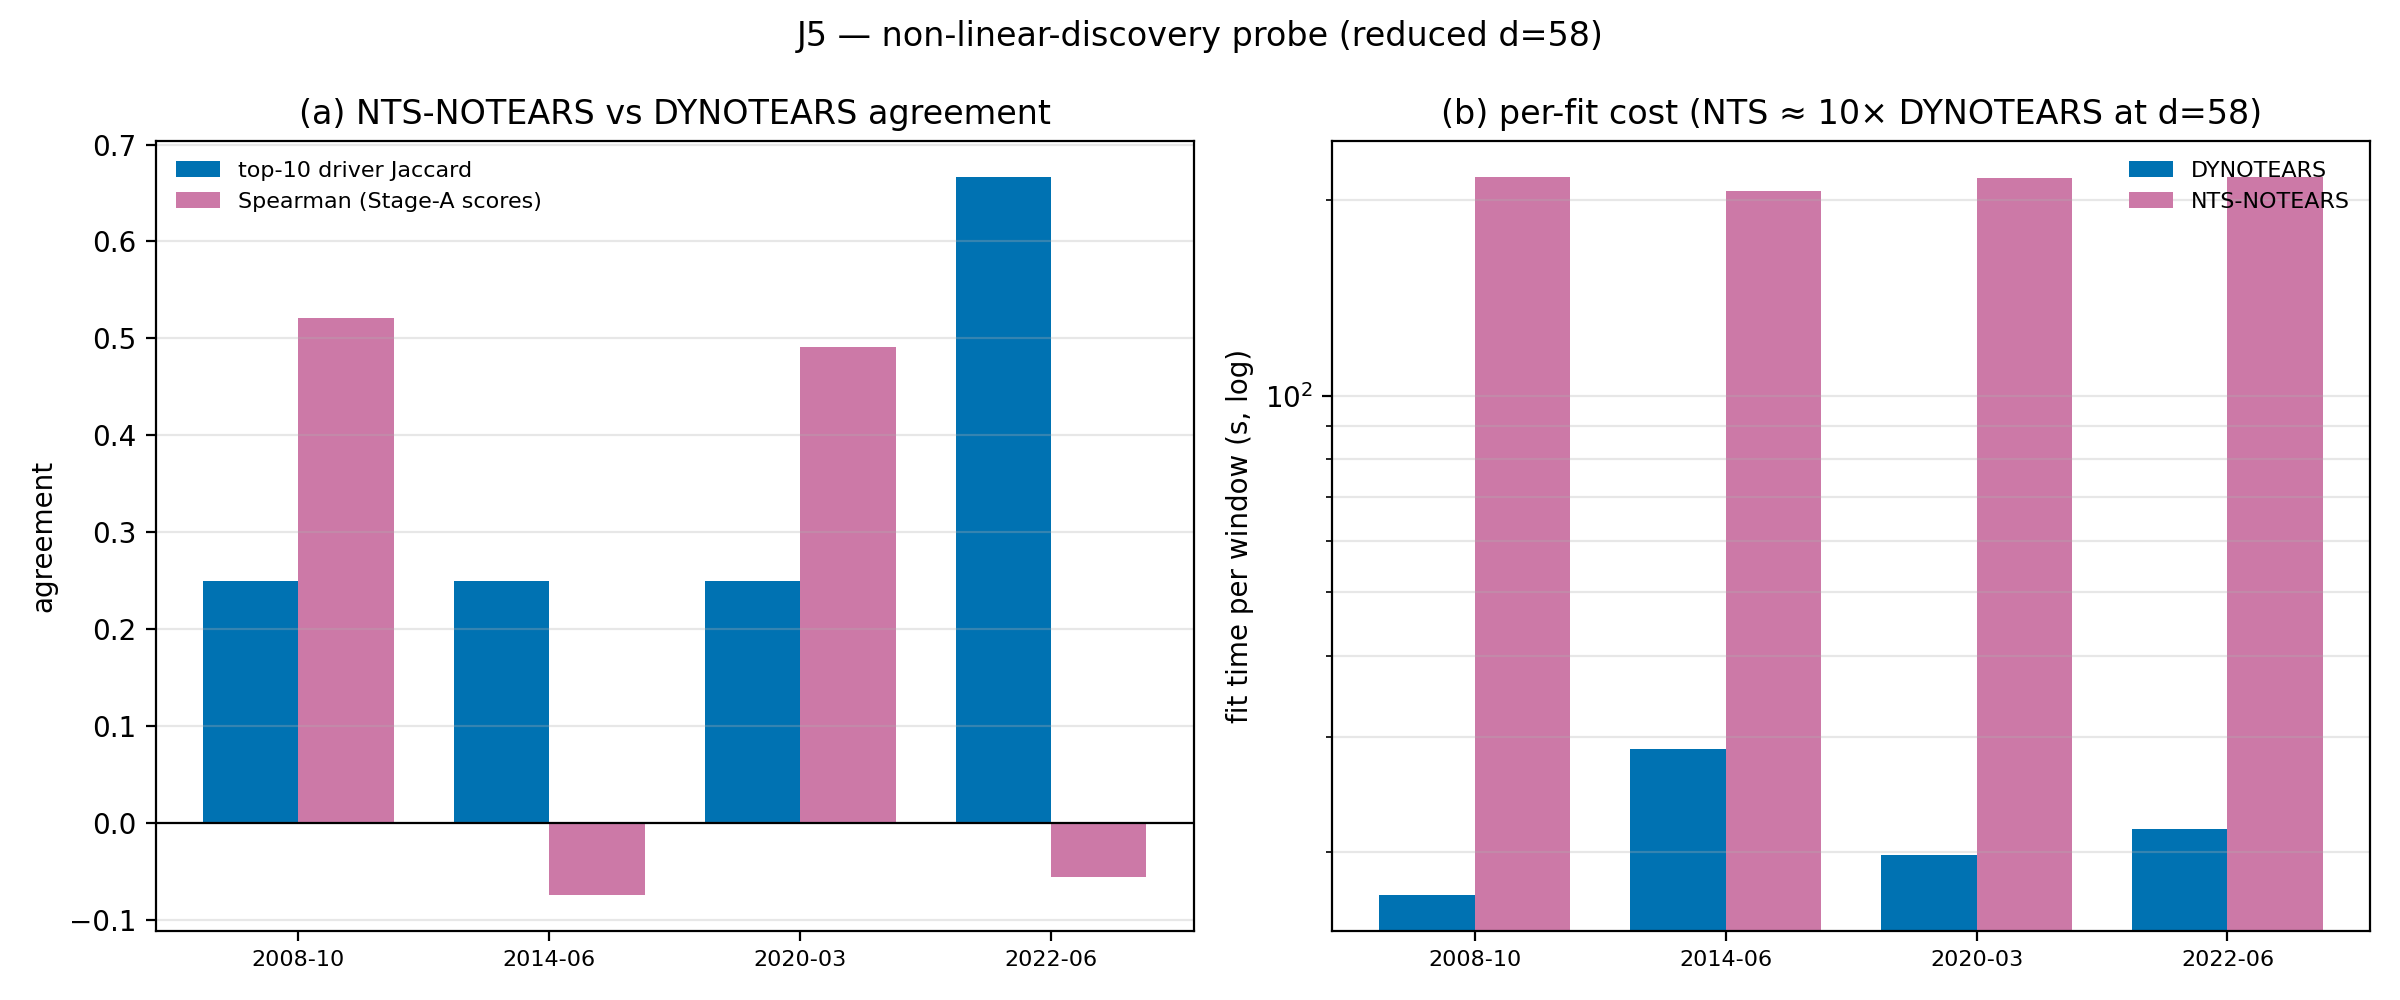
\includegraphics[width=0.95\textwidth]{figures/nts_probe.png}
  \caption{Non-linear-discovery probe (reduced universe $d=58$). (a) Agreement
    between NTS-NOTEARS and DYNOTEARS on driver$\to$asset structure (top-10 driver
    Jaccard and Stage-A score Spearman): modest overall, higher in stress windows.
    (b) Per-window fit cost (log scale): NTS is $\approx 10\times$ DYNOTEARS even
    at this reduced dimension, so a full backtest is left as future work.}
  \label{fig:nts}
\end{figure}

\section{Engineering for tractability and reproducibility}
\label{sec:cache}

Two engineering points are worth recording because they bear on the credibility
of every result in Chapter~\ref{chap:evaluation}.

\paragraph{Discovery cache.} The causal-graph fit is the dominant per-rebalance
cost ($\approx 15$ hours for a 215-rebalance backtest at $d=132$), and it depends
only on the window data and discovery hyperparameters --- \emph{not} on the
number of drivers $K$ or the feedback parameters $\alpha,\gamma$, which act
downstream. A robustness sweep over $K$ or $\alpha,\gamma$ would therefore refit
the identical graph dozens of times. I added a content-keyed disk cache for the
fitted graph (keyed by the exact window content, column set, method and
hyperparameters, with atomic writes), so the first run at each window pays the
fit and every later sweep configuration reuses it. This turned an otherwise
infeasible set of sweeps ($\sim 390$ hours) into roughly two days of wall-clock,
and is what made the K-sensitivity and $\alpha,\gamma$ analyses of
Chapter~\ref{chap:evaluation} possible.

\paragraph{A data-determinism bug, and why it matters.} Building the cache exposed
a latent reproducibility defect. One driver (the emerging-markets ETF EEM, listed
in 2003) had an inception date inside the two-year padding window before the
sample start, so its cache-coverage check never passed and it was silently
re-downloaded from Yahoo Finance on \emph{every} call. With auto-adjustment, the
returned values jittered by $\approx 3\times10^{-7}$ run-to-run, which the
non-convex DYNOTEARS optimiser amplified to changes of $\approx 0.14$ in the
graph $W$. In other words, \emph{the pipeline was not bit-reproducible}, and each
backtest had used a one-off realisation of one driver. I fixed this (reuse a
cached series whenever the previously requested span covers the request; atomic
writes) so that two independent processes now produce byte-identical windows, and
re-ran the entire headline matrix under the corrected, deterministic pipeline.

This is reported prominently for a methodological reason. The fix changed two
headline conclusions: the apparent two-year-window edge of causal selection
collapsed from $+0.012$ to $+0.001$ Sharpe, and an apparent ``significantly worse
closed loop at the two-year window'' ($p=0.031$) disappeared once the feedback was
shown to be exactly inert. A result that does not survive a determinism fix was
never real; finding and correcting this is part of the contribution, and a
reminder that reproducibility is a prerequisite for, not an afterthought to,
empirical claims in this area \cite{lopezdeprado2023causal}.
